% Created by tikzDevice version 0.12.3.1 on 2021-07-01 17:52:09
% !TEX encoding = UTF-8 Unicode
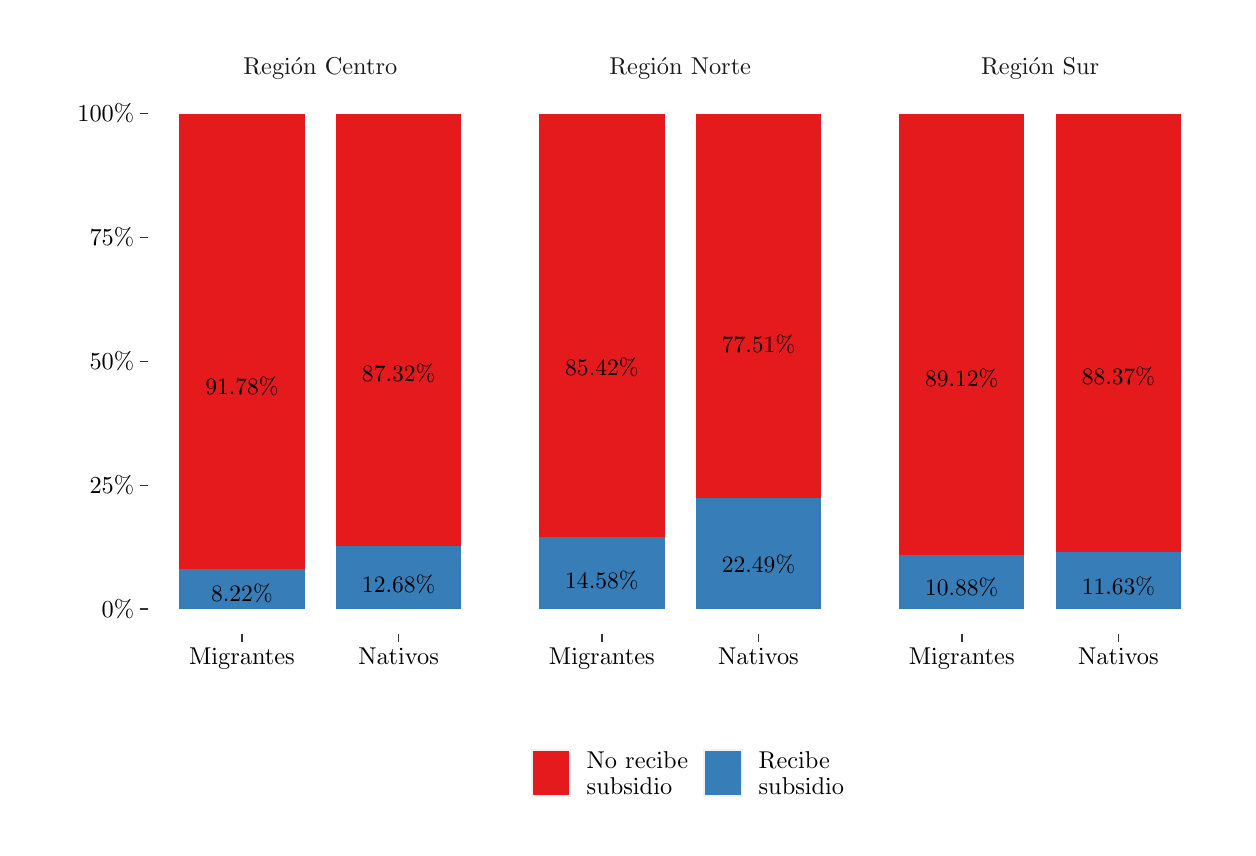
\begin{tikzpicture}[x=1pt,y=1pt]
\definecolor{fillColor}{RGB}{255,255,255}
\path[use as bounding box,fill=fillColor,fill opacity=0.00] (0,0) rectangle (433.62,289.08);
\begin{scope}
\path[clip] (  0.00,  0.00) rectangle (433.62,289.08);
\definecolor{drawColor}{RGB}{255,255,255}
\definecolor{fillColor}{RGB}{255,255,255}

\path[draw=drawColor,line width= 0.6pt,line join=round,line cap=round,fill=fillColor] (  0.00,  0.00) rectangle (433.62,289.08);
\end{scope}
\begin{scope}
\path[clip] ( 43.44, 69.96) rectangle (168.00,267.01);
\definecolor{drawColor}{RGB}{255,255,255}

\path[draw=drawColor,line width= 0.3pt,line join=round] ( 43.44,101.31) --
	(168.00,101.31);

\path[draw=drawColor,line width= 0.3pt,line join=round] ( 43.44,146.09) --
	(168.00,146.09);

\path[draw=drawColor,line width= 0.3pt,line join=round] ( 43.44,190.88) --
	(168.00,190.88);

\path[draw=drawColor,line width= 0.3pt,line join=round] ( 43.44,235.66) --
	(168.00,235.66);

\path[draw=drawColor,line width= 0.6pt,line join=round] ( 43.44, 78.92) --
	(168.00, 78.92);

\path[draw=drawColor,line width= 0.6pt,line join=round] ( 43.44,123.70) --
	(168.00,123.70);

\path[draw=drawColor,line width= 0.6pt,line join=round] ( 43.44,168.48) --
	(168.00,168.48);

\path[draw=drawColor,line width= 0.6pt,line join=round] ( 43.44,213.27) --
	(168.00,213.27);

\path[draw=drawColor,line width= 0.6pt,line join=round] ( 43.44,258.05) --
	(168.00,258.05);

\path[draw=drawColor,line width= 0.6pt,line join=round] ( 77.41, 69.96) --
	( 77.41,267.01);

\path[draw=drawColor,line width= 0.6pt,line join=round] (134.03, 69.96) --
	(134.03,267.01);
\definecolor{fillColor}{RGB}{228,26,28}

\path[fill=fillColor] ( 54.77, 93.64) rectangle (100.06,258.05);
\definecolor{fillColor}{RGB}{55,126,184}

\path[fill=fillColor] ( 54.77, 78.92) rectangle (100.06, 93.64);
\definecolor{fillColor}{RGB}{228,26,28}

\path[fill=fillColor] (111.38,101.64) rectangle (156.68,258.05);
\definecolor{fillColor}{RGB}{55,126,184}

\path[fill=fillColor] (111.38, 78.92) rectangle (156.68,101.64);
\definecolor{drawColor}{RGB}{0,0,0}

\node[text=drawColor,anchor=base,inner sep=0pt, outer sep=0pt, scale=  0.85] at ( 77.41,156.47) {91.78{\%}};

\node[text=drawColor,anchor=base,inner sep=0pt, outer sep=0pt, scale=  0.85] at ( 77.41, 81.87) {8.22{\%}};

\node[text=drawColor,anchor=base,inner sep=0pt, outer sep=0pt, scale=  0.85] at (134.03,161.26) {87.32{\%}};

\node[text=drawColor,anchor=base,inner sep=0pt, outer sep=0pt, scale=  0.85] at (134.03, 85.07) {12.68{\%}};
\end{scope}
\begin{scope}
\path[clip] (173.50, 69.96) rectangle (298.06,267.01);
\definecolor{drawColor}{RGB}{255,255,255}

\path[draw=drawColor,line width= 0.3pt,line join=round] (173.50,101.31) --
	(298.06,101.31);

\path[draw=drawColor,line width= 0.3pt,line join=round] (173.50,146.09) --
	(298.06,146.09);

\path[draw=drawColor,line width= 0.3pt,line join=round] (173.50,190.88) --
	(298.06,190.88);

\path[draw=drawColor,line width= 0.3pt,line join=round] (173.50,235.66) --
	(298.06,235.66);

\path[draw=drawColor,line width= 0.6pt,line join=round] (173.50, 78.92) --
	(298.06, 78.92);

\path[draw=drawColor,line width= 0.6pt,line join=round] (173.50,123.70) --
	(298.06,123.70);

\path[draw=drawColor,line width= 0.6pt,line join=round] (173.50,168.48) --
	(298.06,168.48);

\path[draw=drawColor,line width= 0.6pt,line join=round] (173.50,213.27) --
	(298.06,213.27);

\path[draw=drawColor,line width= 0.6pt,line join=round] (173.50,258.05) --
	(298.06,258.05);

\path[draw=drawColor,line width= 0.6pt,line join=round] (207.47, 69.96) --
	(207.47,267.01);

\path[draw=drawColor,line width= 0.6pt,line join=round] (264.09, 69.96) --
	(264.09,267.01);
\definecolor{fillColor}{RGB}{228,26,28}

\path[fill=fillColor] (184.83,105.04) rectangle (230.12,258.05);
\definecolor{fillColor}{RGB}{55,126,184}

\path[fill=fillColor] (184.83, 78.92) rectangle (230.12,105.04);
\definecolor{fillColor}{RGB}{228,26,28}

\path[fill=fillColor] (241.44,119.20) rectangle (286.74,258.05);
\definecolor{fillColor}{RGB}{55,126,184}

\path[fill=fillColor] (241.44, 78.92) rectangle (286.74,119.20);
\definecolor{drawColor}{RGB}{0,0,0}

\node[text=drawColor,anchor=base,inner sep=0pt, outer sep=0pt, scale=  0.85] at (207.47,163.30) {85.42{\%}};

\node[text=drawColor,anchor=base,inner sep=0pt, outer sep=0pt, scale=  0.85] at (207.47, 86.43) {14.58{\%}};

\node[text=drawColor,anchor=base,inner sep=0pt, outer sep=0pt, scale=  0.85] at (264.09,171.80) {77.51{\%}};

\node[text=drawColor,anchor=base,inner sep=0pt, outer sep=0pt, scale=  0.85] at (264.09, 92.09) {22.49{\%}};
\end{scope}
\begin{scope}
\path[clip] (303.56, 69.96) rectangle (428.12,267.01);
\definecolor{drawColor}{RGB}{255,255,255}

\path[draw=drawColor,line width= 0.3pt,line join=round] (303.56,101.31) --
	(428.12,101.31);

\path[draw=drawColor,line width= 0.3pt,line join=round] (303.56,146.09) --
	(428.12,146.09);

\path[draw=drawColor,line width= 0.3pt,line join=round] (303.56,190.88) --
	(428.12,190.88);

\path[draw=drawColor,line width= 0.3pt,line join=round] (303.56,235.66) --
	(428.12,235.66);

\path[draw=drawColor,line width= 0.6pt,line join=round] (303.56, 78.92) --
	(428.12, 78.92);

\path[draw=drawColor,line width= 0.6pt,line join=round] (303.56,123.70) --
	(428.12,123.70);

\path[draw=drawColor,line width= 0.6pt,line join=round] (303.56,168.48) --
	(428.12,168.48);

\path[draw=drawColor,line width= 0.6pt,line join=round] (303.56,213.27) --
	(428.12,213.27);

\path[draw=drawColor,line width= 0.6pt,line join=round] (303.56,258.05) --
	(428.12,258.05);

\path[draw=drawColor,line width= 0.6pt,line join=round] (337.53, 69.96) --
	(337.53,267.01);

\path[draw=drawColor,line width= 0.6pt,line join=round] (394.15, 69.96) --
	(394.15,267.01);
\definecolor{fillColor}{RGB}{228,26,28}

\path[fill=fillColor] (314.88, 98.41) rectangle (360.18,258.05);
\definecolor{fillColor}{RGB}{55,126,184}

\path[fill=fillColor] (314.88, 78.92) rectangle (360.18, 98.41);
\definecolor{fillColor}{RGB}{228,26,28}

\path[fill=fillColor] (371.50, 99.76) rectangle (416.80,258.05);
\definecolor{fillColor}{RGB}{55,126,184}

\path[fill=fillColor] (371.50, 78.92) rectangle (416.80, 99.76);
\definecolor{drawColor}{RGB}{0,0,0}

\node[text=drawColor,anchor=base,inner sep=0pt, outer sep=0pt, scale=  0.85] at (337.53,159.33) {89.12{\%}};

\node[text=drawColor,anchor=base,inner sep=0pt, outer sep=0pt, scale=  0.85] at (337.53, 83.77) {10.88{\%}};

\node[text=drawColor,anchor=base,inner sep=0pt, outer sep=0pt, scale=  0.85] at (394.15,160.14) {88.37{\%}};

\node[text=drawColor,anchor=base,inner sep=0pt, outer sep=0pt, scale=  0.85] at (394.15, 84.31) {11.63{\%}};
\end{scope}
\begin{scope}
\path[clip] ( 43.44,267.01) rectangle (168.00,283.58);
\definecolor{drawColor}{gray}{0.10}

\node[text=drawColor,anchor=base,inner sep=0pt, outer sep=0pt, scale=  0.88] at (105.72,272.26) {Región Centro};
\end{scope}
\begin{scope}
\path[clip] (173.50,267.01) rectangle (298.06,283.58);
\definecolor{drawColor}{gray}{0.10}

\node[text=drawColor,anchor=base,inner sep=0pt, outer sep=0pt, scale=  0.88] at (235.78,272.26) {Región Norte};
\end{scope}
\begin{scope}
\path[clip] (303.56,267.01) rectangle (428.12,283.58);
\definecolor{drawColor}{gray}{0.10}

\node[text=drawColor,anchor=base,inner sep=0pt, outer sep=0pt, scale=  0.88] at (365.84,272.26) {Región Sur};
\end{scope}
\begin{scope}
\path[clip] (  0.00,  0.00) rectangle (433.62,289.08);
\definecolor{drawColor}{gray}{0.20}

\path[draw=drawColor,line width= 0.6pt,line join=round] ( 77.41, 67.21) --
	( 77.41, 69.96);

\path[draw=drawColor,line width= 0.6pt,line join=round] (134.03, 67.21) --
	(134.03, 69.96);
\end{scope}
\begin{scope}
\path[clip] (  0.00,  0.00) rectangle (433.62,289.08);
\definecolor{drawColor}{RGB}{0,0,0}

\node[text=drawColor,anchor=base,inner sep=0pt, outer sep=0pt, scale=  0.88] at ( 77.41, 58.95) {Migrantes};

\node[text=drawColor,anchor=base,inner sep=0pt, outer sep=0pt, scale=  0.88] at (134.03, 58.95) {Nativos};
\end{scope}
\begin{scope}
\path[clip] (  0.00,  0.00) rectangle (433.62,289.08);
\definecolor{drawColor}{gray}{0.20}

\path[draw=drawColor,line width= 0.6pt,line join=round] (207.47, 67.21) --
	(207.47, 69.96);

\path[draw=drawColor,line width= 0.6pt,line join=round] (264.09, 67.21) --
	(264.09, 69.96);
\end{scope}
\begin{scope}
\path[clip] (  0.00,  0.00) rectangle (433.62,289.08);
\definecolor{drawColor}{RGB}{0,0,0}

\node[text=drawColor,anchor=base,inner sep=0pt, outer sep=0pt, scale=  0.88] at (207.47, 58.95) {Migrantes};

\node[text=drawColor,anchor=base,inner sep=0pt, outer sep=0pt, scale=  0.88] at (264.09, 58.95) {Nativos};
\end{scope}
\begin{scope}
\path[clip] (  0.00,  0.00) rectangle (433.62,289.08);
\definecolor{drawColor}{gray}{0.20}

\path[draw=drawColor,line width= 0.6pt,line join=round] (337.53, 67.21) --
	(337.53, 69.96);

\path[draw=drawColor,line width= 0.6pt,line join=round] (394.15, 67.21) --
	(394.15, 69.96);
\end{scope}
\begin{scope}
\path[clip] (  0.00,  0.00) rectangle (433.62,289.08);
\definecolor{drawColor}{RGB}{0,0,0}

\node[text=drawColor,anchor=base,inner sep=0pt, outer sep=0pt, scale=  0.88] at (337.53, 58.95) {Migrantes};

\node[text=drawColor,anchor=base,inner sep=0pt, outer sep=0pt, scale=  0.88] at (394.15, 58.95) {Nativos};
\end{scope}
\begin{scope}
\path[clip] (  0.00,  0.00) rectangle (433.62,289.08);
\definecolor{drawColor}{RGB}{0,0,0}

\node[text=drawColor,anchor=base east,inner sep=0pt, outer sep=0pt, scale=  0.88] at ( 38.49, 75.89) {0{\%}};

\node[text=drawColor,anchor=base east,inner sep=0pt, outer sep=0pt, scale=  0.88] at ( 38.49,120.67) {25{\%}};

\node[text=drawColor,anchor=base east,inner sep=0pt, outer sep=0pt, scale=  0.88] at ( 38.49,165.45) {50{\%}};

\node[text=drawColor,anchor=base east,inner sep=0pt, outer sep=0pt, scale=  0.88] at ( 38.49,210.24) {75{\%}};

\node[text=drawColor,anchor=base east,inner sep=0pt, outer sep=0pt, scale=  0.88] at ( 38.49,255.02) {100{\%}};
\end{scope}
\begin{scope}
\path[clip] (  0.00,  0.00) rectangle (433.62,289.08);
\definecolor{drawColor}{gray}{0.20}

\path[draw=drawColor,line width= 0.6pt,line join=round] ( 40.69, 78.92) --
	( 43.44, 78.92);

\path[draw=drawColor,line width= 0.6pt,line join=round] ( 40.69,123.70) --
	( 43.44,123.70);

\path[draw=drawColor,line width= 0.6pt,line join=round] ( 40.69,168.48) --
	( 43.44,168.48);

\path[draw=drawColor,line width= 0.6pt,line join=round] ( 40.69,213.27) --
	( 43.44,213.27);

\path[draw=drawColor,line width= 0.6pt,line join=round] ( 40.69,258.05) --
	( 43.44,258.05);
\end{scope}
\begin{scope}
\path[clip] (  0.00,  0.00) rectangle (433.62,289.08);
\definecolor{fillColor}{RGB}{255,255,255}

\path[fill=fillColor] (171.04,  5.50) rectangle (300.52, 33.78);
\end{scope}
\begin{scope}
\path[clip] (  0.00,  0.00) rectangle (433.62,289.08);
\definecolor{fillColor}{gray}{0.95}

\path[fill=fillColor] (182.04, 11.00) rectangle (196.50, 28.28);
\end{scope}
\begin{scope}
\path[clip] (  0.00,  0.00) rectangle (433.62,289.08);
\definecolor{fillColor}{RGB}{228,26,28}

\path[fill=fillColor] (182.75, 11.71) rectangle (195.78, 27.56);
\end{scope}
\begin{scope}
\path[clip] (  0.00,  0.00) rectangle (433.62,289.08);
\definecolor{fillColor}{gray}{0.95}

\path[fill=fillColor] (244.18, 11.00) rectangle (258.63, 28.28);
\end{scope}
\begin{scope}
\path[clip] (  0.00,  0.00) rectangle (433.62,289.08);
\definecolor{fillColor}{RGB}{55,126,184}

\path[fill=fillColor] (244.89, 11.71) rectangle (257.92, 27.56);
\end{scope}
\begin{scope}
\path[clip] (  0.00,  0.00) rectangle (433.62,289.08);
\definecolor{drawColor}{RGB}{0,0,0}

\node[text=drawColor,anchor=base west,inner sep=0pt, outer sep=0pt, scale=  0.88] at (202.00, 21.36) {No recibe};

\node[text=drawColor,anchor=base west,inner sep=0pt, outer sep=0pt, scale=  0.88] at (202.00, 11.86) {subsidio};
\end{scope}
\begin{scope}
\path[clip] (  0.00,  0.00) rectangle (433.62,289.08);
\definecolor{drawColor}{RGB}{0,0,0}

\node[text=drawColor,anchor=base west,inner sep=0pt, outer sep=0pt, scale=  0.88] at (264.13, 21.36) {Recibe};

\node[text=drawColor,anchor=base west,inner sep=0pt, outer sep=0pt, scale=  0.88] at (264.13, 11.86) {subsidio};
\end{scope}
\end{tikzpicture}
